Urban areas are highly complex environments which introduce numerous challenges
to autonomous service robots. In particular, for a safe and reliable navigation,
a robot should be able to accurately detect curbs. Curbs usually appear at the
borders between streets and sidewalks. The knowledge of curb positions and
characteristics can beneficially enhance metric maps with traversability
informations relevant to navigation. For instance, a robotic platform could only
navigate harmlessly over curbs of a certain height when crossing a street.

Amongst the difficulties related to this task, curbs might exhibit various
curvatures and heights, and be perceived from different viewpoints. Furthermore,
the sensing device noise model should be introduced to distinguish between real
curbs and measurement noise. Ideally, the algorithm should run on-line and
real-time.

In this paper, we devise an unsupervised method to curb detection that covers
most of the aforementioned requirements. Our approach attempts to construct a
piecewise planar model of the environment and determines curbs at plane segment
boundaries. Initially, we sense the environment with a nodding laser
range-finder and project the 3D measurements into an efficient Digital Elevation
Map (DEM). Each cell of the DEM maintains an error model that is propagated
throughout the entire algorithm. Plane segments are further estimated with a
mixture of linear regressions on the DEM. Here, we propose an original
formulation of the standard Expectation-Maximization (EM) algorithm for mixture
models. Specifically, in the E-step, the responsibilities are computed with a
Conditional Random Field (CRF), that smooths the assignment of DEM cells to
planes of the mixture model. An initial graph-based segmentation of the DEM
provides the first responsibilities and an estimate of the number of planes.
Fig.~\ref{fig:intro} shows a typical output of our algorithm.

\begin{figure}[t]
\centering
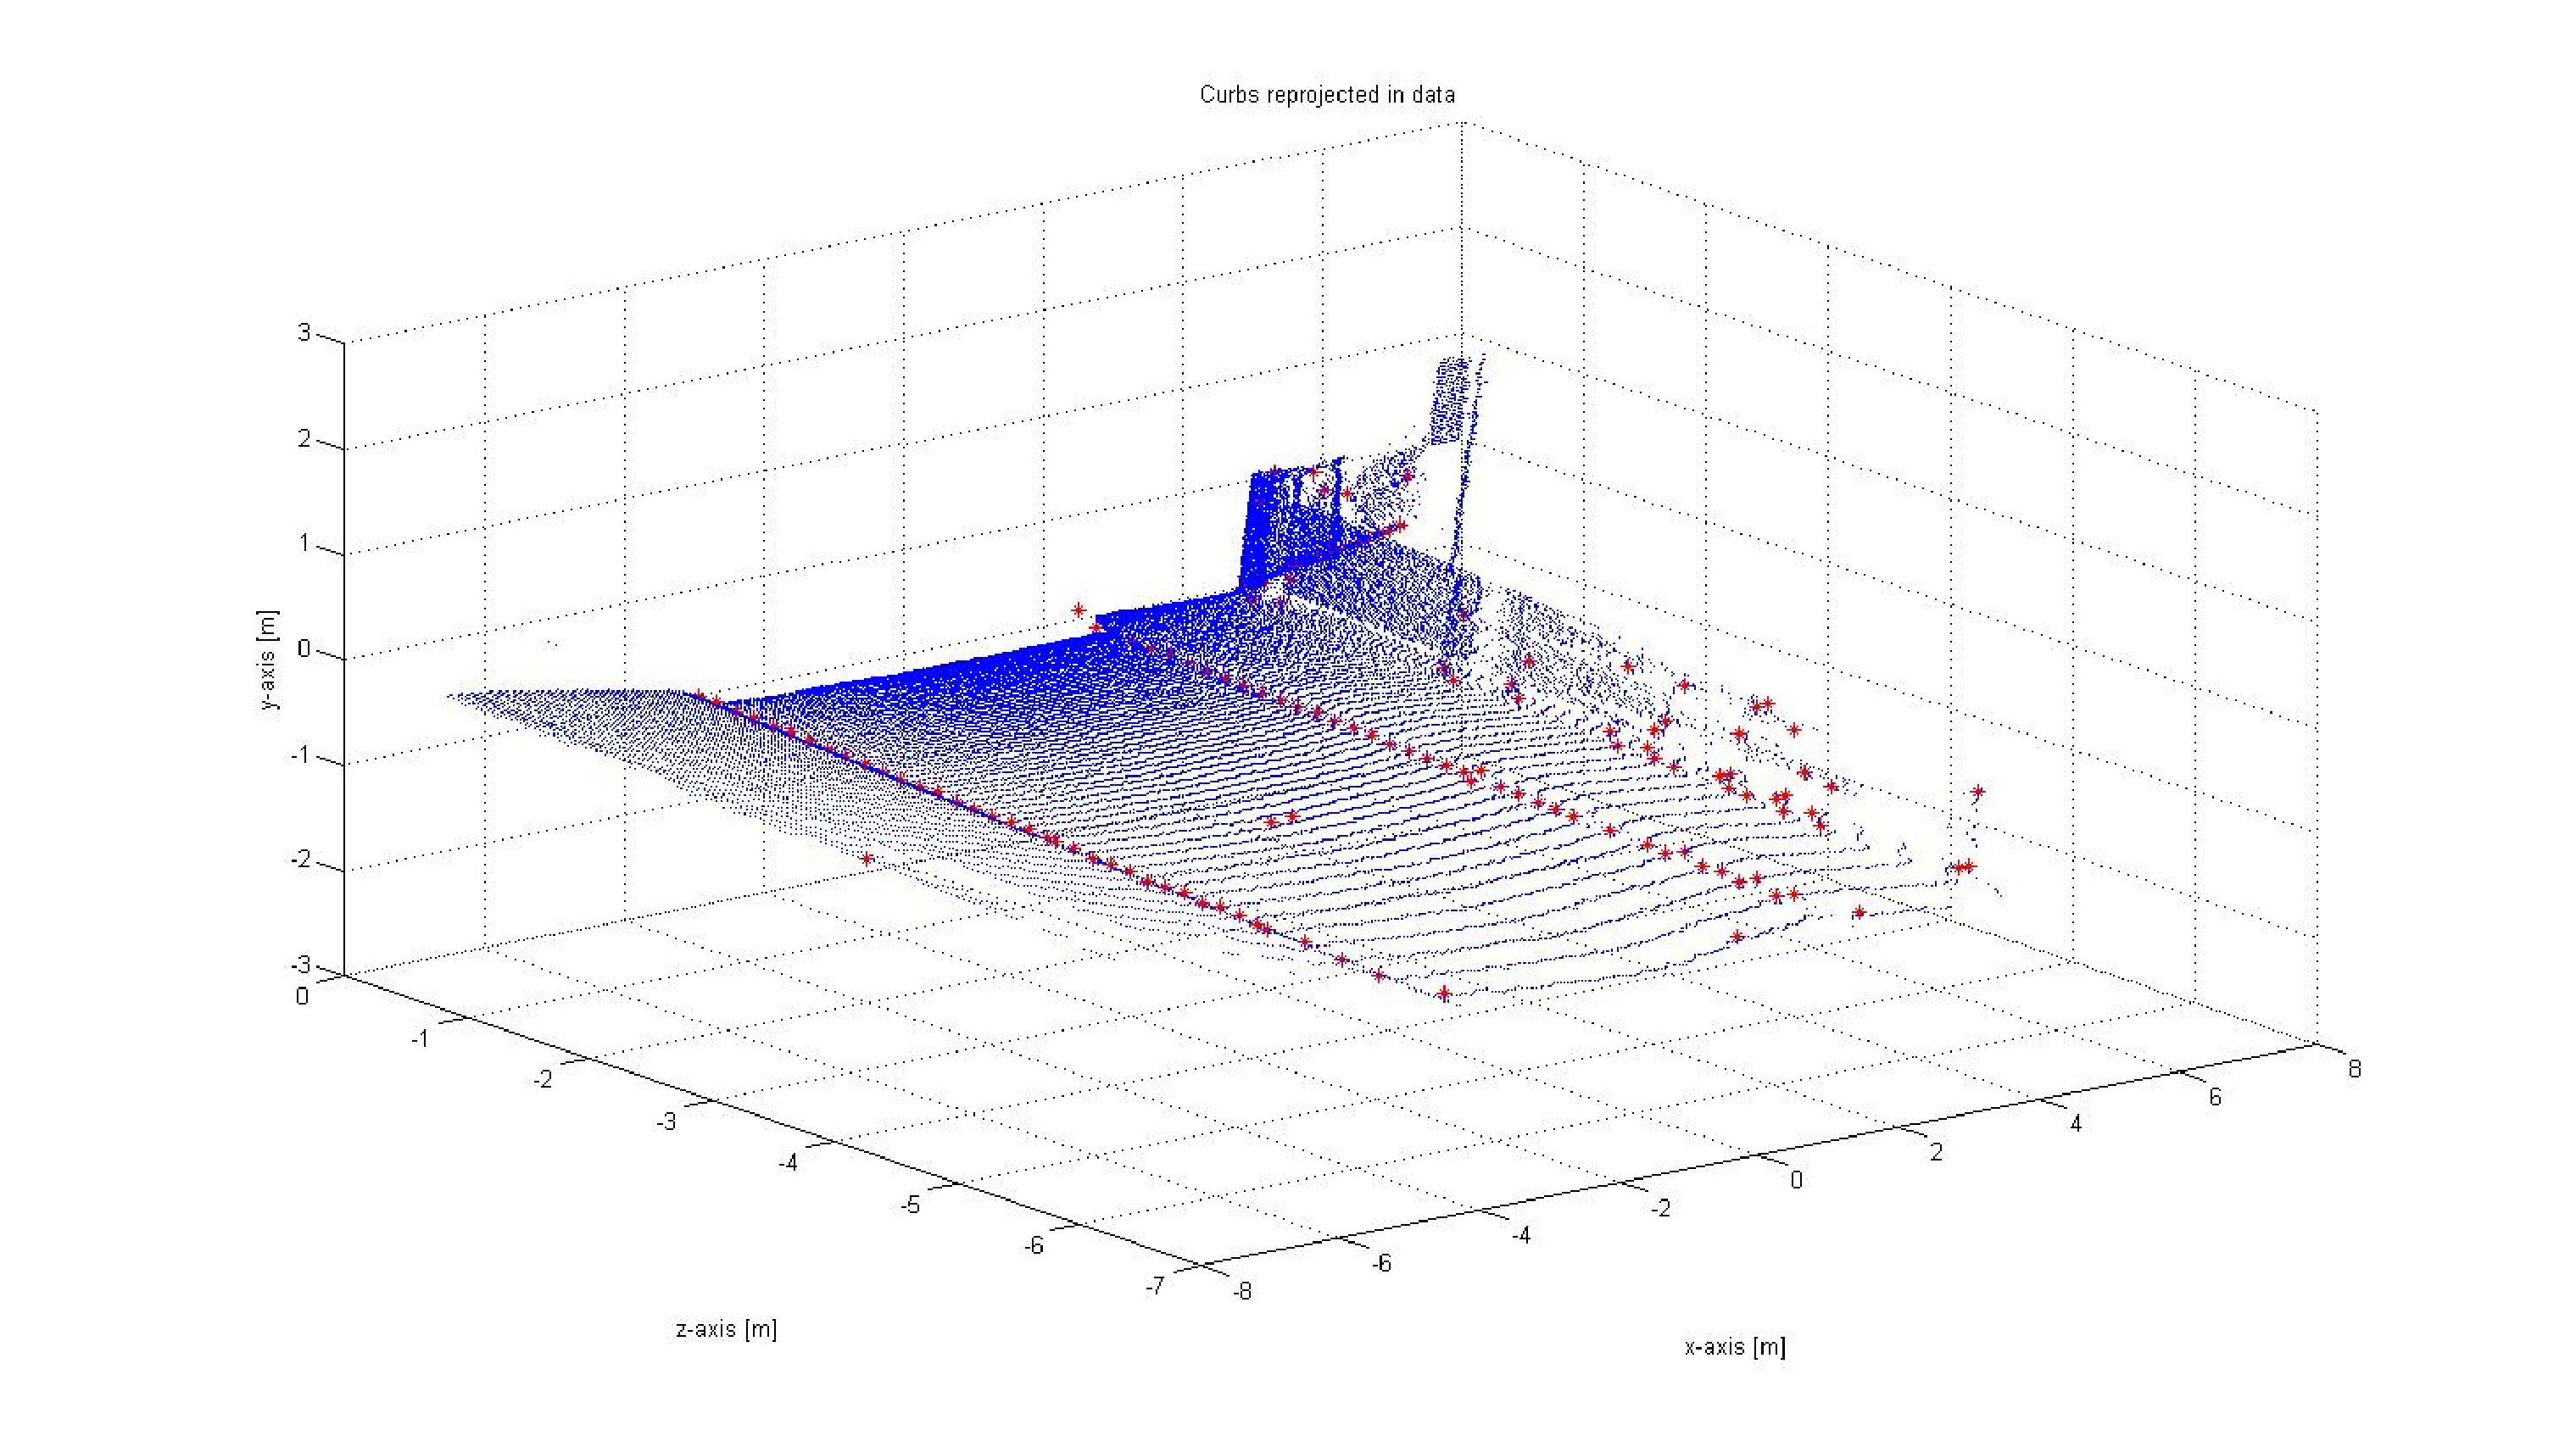
\includegraphics[width=\columnwidth]{fig/intro.eps}
\caption{Exemplary output of our curb detection algorithm. Curb points
(red stars) are reprojected into the original point cloud.}
\label{fig:intro}
\end{figure}

Clearly, the strength of the paper is its strict probabilistic justification
from the sensing device to the final plane segmentation and estimation.
Moreover, it makes few assumptions about the environment and limits the number
of hand-tuned parameters. Finally, the algorithm should hopefully be easy to
implement from the paper.

The remainder of the paper is structured as follows. Section~\ref{sec:related}
summarizes the previous works related to ours. Section~\ref{sec:model}
introduces our notations and models. Section~\ref{sec:initial} describes the
graph-based segmentation for initial labeling. Section~\ref{sec:plane} derives
the weighted plane regression. Section~\ref{sec:crf} presents the CRF for
global DEM cell labeling. Section~\ref{sec:exp} demonstrates experimental
results. Section~\ref{sec:conc} outlines our conclusions and provides some
insights for future work.
